\documentclass[twocolumn]{article}

\usepackage{mathtools}
\usepackage{amsmath,amsfonts}
\usepackage{lscape}
\usepackage{bm}
\usepackage{breqn}
\usepackage{hyperref}


\usepackage{graphicx}
\usepackage[utf8]{inputenc}

\usepackage{tikz}
\usetikzlibrary{shapes.geometric,calc}
\usetikzlibrary{patterns}

\usepackage{natbib}

\tikzset{
pro/.style={circle,draw=black,fill=none,inner sep=1pt,minimum size=1.3em},
sil/.style={circle,draw=none,fill=black,inner sep=0pt,minimum size=5pt}
}

\DeclareBoldMathCommand{\t}{t}
\DeclareMathOperator{\loss}{\ell}
\newcommand{\segs}{\mathbb S}
\newcommand{\head}{\mathcal H}
\newcommand{\tail}{\mathcal T}
\newcommand{\best}{\mathcal V}

\usepackage{multirow}
\usepackage{array}
\usepackage{colortbl}

\newlength\epaisLigne
\newcommand\Mline[2]{\noalign{\global\epaisLigne\arrayrulewidth\global\arrayrulewidth#1pt}\cline{#2}\noalign{\global\arrayrulewidth\epaisLigne}}

%\newcommand{\mynote}[1]{\marginpar{\tiny #1}}
\newcommand{\mynote}[1]{}

\hypersetup{
	pdfauthor={Tim Scarfe, Wouter M. Koolen and Yuri Kalnishkan},
	pdftitle={Segmenting electronic dance music streams based on self-similarity},
pdfkeywords={audio,stream,segmentation,dj,mixing},
pdfsubject={Artificial Intelligence},
pdfcreator={Tim Scarfe},
pdfproducer={Tim Scarfe},
}
\title{
A long-range self-similarity approach to segmenting DJ mixed music streams}
\author{Tim Scarfe, Wouter M.~Koolen and Yuri Kalnishkan \\ 
Computer Learning Research
 Centre and Department of Computer Science, \\ 
Royal Holloway,  University of London, Egham, Surrey, TW20 0EX, United Kingdom\\
\{tim,wouter,yura\}@cs.rhul.ac.uk
}

\pagestyle{plain}
% to remove in the final version!!


%\renewcommand*{\algorithmcfname}{Protocol}
% see http://tex.stackexchange.com/questions/22477/renaming-algorithm-to-heuristic-in-algorithm2e-package


\title{Segmenting electronic dance music streams based on self-similarity}
\begin{document}

\maketitle

\begin{abstract}

We describe an unsupervised, deterministic algorithm for segmenting DJ-mixed Electronic Dance Music (EDM) streams (for example; pod-casts, radio shows, live events) into their respective tracks. We attempt to reconstruct boundaries as close as possible to what a human domain expert would create in respect of the same task. The goal of DJ-mixing is to render track boundaries effectively invisible from the standpoint of human perception which makes the problem difficult.

We use dynamic programming to optimally segment a cost matrix derived from a similarity matrix. The similarity matrix is based on the cosines of a time series of kernel-transformed Fourier based features designed with this domain in mind. Our method is applied to EDM streams. Its formulation incorporates long-term self similarity as a first class concept combined with dynamic programming and it is qualitatively assessed on a large corpus of long streams that have been hand labelled by a domain expert.
\smallskip

\noindent \textbf{Keywords.} \noindent music,segmentation,DJ mix,dynamic programming

\end{abstract}


\vspace{1em}

\section{Introduction}

Electronic Dance Music tracks are usually mixed by a DJ, which sets EDM streams apart from other genres of music. Mixing is the \textit{modus operandi} in electronic music. We first transform the audio file into a time series of features (grouped into tiles) and transform those tiles into a domain where any pair from the same track would be distinguishable by their cosine. Our features are based on a Fourier transform with kernel filtering to accentuate instruments and intended self-similarity. We create a similarity matrix from these cosines and then derive a cost matrix showing the costs of fitting a track at a given time with a given width. We use Dynamic Programming (DP) to create the cost matrix and again to perform the most economical segmentation of the cost matrix to fit a predetermined number of tracks.

A distinguishing feature of our algorithm is that it focuses on long term self similarity of segments rather than short term transients. Dance music tracks have the property that they are made up of repeating regions, and the ends are almost always similar to the beginning. For this reason we believe that some techniques from structural analysis fail to perform as well for this segmentation task because we focus on the concept of self-similarity ranging over a customisable time horizon. Our method does not require any training or tenuous heuristics to perform well. 

The purpose of this algorithm is to reconstruct boundaries given a fixed number of tracks known in advance (their names and order are known). This is relevant when one has recorded a show, downloaded a track list and needs to reconstruct the indices given a track list. The order of the indices reconstructed is critical so that we can align the correct track names with the reconstructed indices. If the track list was not known in advance the number of tracks could be estimated in most cases.

One of the interesting features of audio is that you \textit{can not scrub through it and get an overview in the same way you can with video}. Audio does not have the same \textit{contextual continuum} when the user skips through it perhaps due to the lack of redundant, persistent scene-setting information. Metadata would allow click through monetisation, and allow improved use-case scenarios (for example publishing to social networks, information discovery and retrieval). Capturing metadata in audio is a time consuming process. Tzanetakis found in \cite{tzanetakis1999framework} that it took users on average $2$ hours to segment $10$ minutes of audio using standard tools. While not directly relevant we might glean from those findings that there is a strong motivation to automate this process. 

To mix tracks DJs always match the speed or \textit{BPM} (beats per minute) of each adjacent track during a transition and align the major percussive elements in the time domain. This is the central concept of removing any dissonance from overlapping tracks. Tracks can overlap by any amount. DJs increase adjacent track compatibility further by selecting adjacent pairs that are harmonically compatible and by applying spectral transformations (EQ).
 
The main theme of the early literature was attempting to generate a novelty function to find points of change using distance-based metrics or statistical methods. Heuristic methods with hard decision boundaries were used to find the best peaks. A distinguishing feature of our approach is that we evaluate how well we are doing compared to humans for the same task. We compare our reconstructed indices to the ones created by a human domain expert. 

J.\ Foote et al \citep{foote1999visualizing,foote1997similarity,foote2000automatic,foote2003media,foote2001visualizing} have done a significant amount of work in this area and the first to use similarity matrices. Foote evaluated a Gaussian tapered checkerboard kernel along the diagonal of a similarity matrix to create a 1d novelty function. One benefit to our approach is that our DP allows any range of long-term self similarity (which relates to the fixed kernel size in Foote's work).

Goodwin et al.\ also used DP for segmentation \citep{goodwin2003audio,goodwin2004dynamic}. Their intriguing supervised approach was to perform Linear Discriminant Analysis (LDA) on the features to transform them into a domain where segmentation boundaries would be emphasised and the feature weights normalised. They then reformulated the problem into a clustering DP to find an arbitrary number of clusters. We believe the frame of mind for this work was structural analysis, because it focuses on short term transients (mitigated slightly by the LDA) and would find segments between two regions of long term self similarity. Goodwin was the first to discuss the shortcomings of novelty peak finding approaches. Goodwin's approach is not optimized to work for a predetermined number of segments and depends on the parametrization and training of the LDA transform. 

Peeters et al \citep{peeters2002toward,peeters2004deriving} did some interesting work combining k-means and a transformation of the segmentation problem into Viterbi (a dynamic program).

We compare our error to the relative error of cue sheets created by human domain experts. We focus directly on DJ mixed electronic dance music.

In the coming sections we will describe the data set (Sect.~\ref{dataset}), the evaluation criteria (Sect.~\ref{eval_crit}), the test set (Sect.~\ref{test_set}), data preprocessing (Sect.~\ref{proprocessing}), feature extraction (Sect.~\ref{feat_ex}), cost matrix (Sect.~\ref{costmatrix_sec}), computing the best segmentation (Sect.~\ref{best_cost}), experiment methodology and results (Sect.~\ref{results_sec}), ideas to improve the cost matrix (Sect.~\ref{sec:improved-cost-function-ideas}) and finally the Summary (Sect.~\ref{conclusions}).

I would like to personally thank Mikael Lindgren and Dennis Goncharov from cuenation\footnote{\url{http://www.cuenation.com}} for their help explaining how they make cues and for providing the data set to test the algorithm on.



\begin{figure}[htb]
\centering
  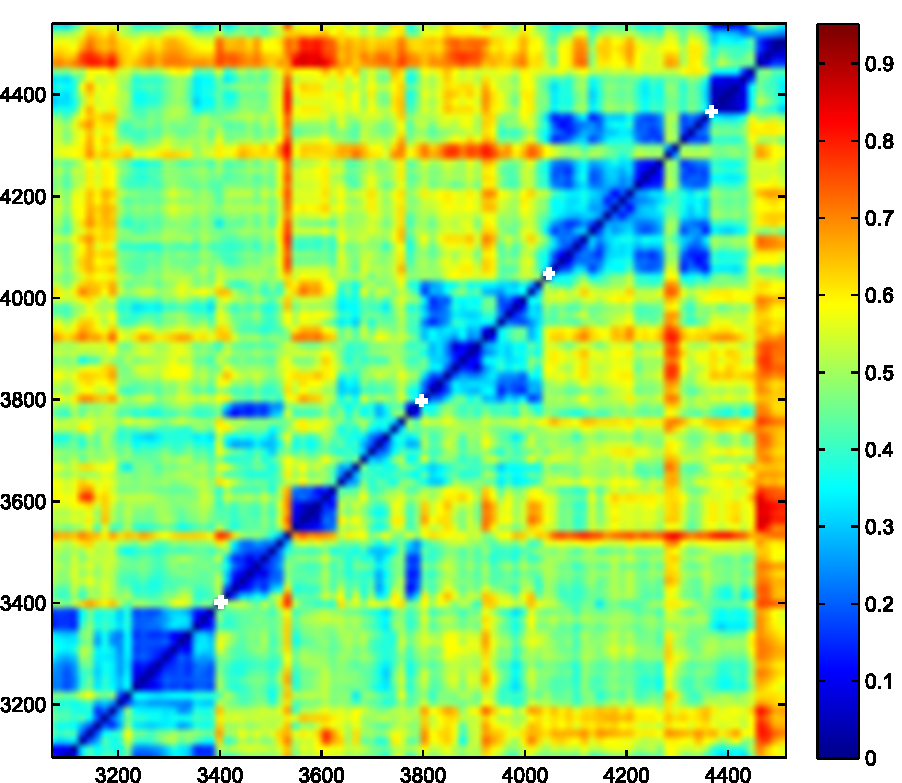
\includegraphics[width= \linewidth]{images/simmat_nopreds.pdf}
      \caption{An example of the similarity matrix S. The second song in this image has an interesting region structure $\{ABCDA\}$. Songs that have so many independent sub regions can be a problem for the cost matrix heuristic which simply sums the cells.}
    \end{figure}
    
    \begin{figure}[htb]
    \centering
         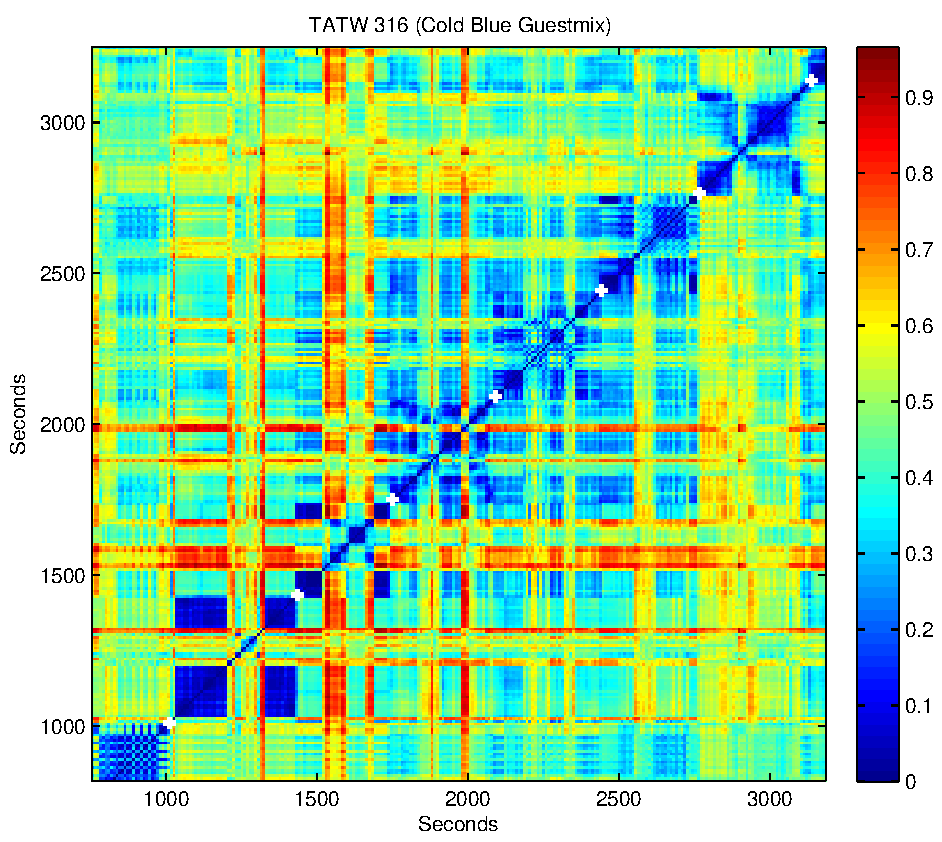
\includegraphics[width= \linewidth]{images/simmat_hardexample.pdf}
       \caption{A complex example of the similarity matrix S. This is an example of a very difficult segmentation task. This similarity matrix represents the domain of instrument features. In this example the boundaries between the tracks are hard to distinguish because adjacent tracks share the same instruments. This might imply that they are by the same artist (lazy artists) or a DJ trying to impress by mixing harmonically and creating shared instrumental features across groups of tracks.}
        \end{figure}
    



\section{Data Set}\label{dataset}

We have been supplied with several broadcasts from three popular radio shows. These are: Magic Island, by Roger Shah ($108$ shows); A State of Trance with Armin Van Buuren ($110$ shows); and Trance Around The World with Above and Beyond ($99$ shows) (Total $317$ shows). The show genres are a mix of Progressive Trance, Uplifting Trance and Tech-Trance. We believe this corpus is the largest of its kind used \cite{peiszer2008automatic} in the literature.  
The music remains uninterrupted after the introduction (no silent gaps). 
The shows come in $44100$ samples per second, $16$ bit stereo MP3 files sampled at $192$Kbs. We resampled these to $4000$Hz $16$ bit mono (left+right channel) WAV files to allow us to process them faster. We have used the ``Sound eXchange''\footnote{\url{http://sox.sourceforge.net}}  program to do this. These shows are all $2$ hours long. The overall average track length is $5$ and a half minutes and normally distributed. The average number of tracks is $23$ for ASOT and TATW, $19$ for Magic Island. There is a guest mix on the second half of each show. The guest mix DJs show off their skills with some of the most technically convoluted mixing imaginable.

\begin{figure}
\centering
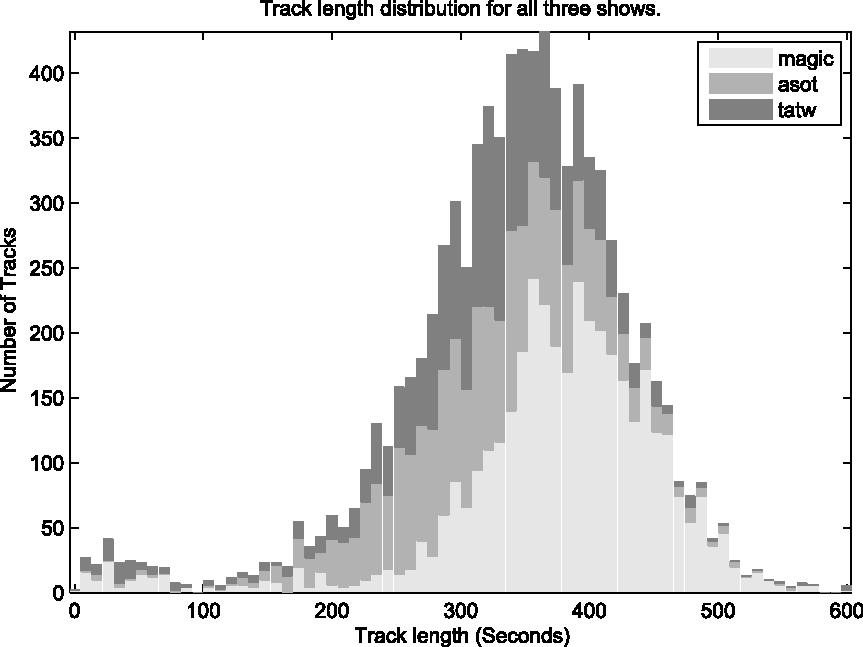
\includegraphics[width=0.45\textwidth]{images/tracklength.pdf}

\caption{The track length distribution for all three radio shows. The \textit{bump} of short tracks (less than $3$ minutes) are often introductions and are manifestly not normal. We removed all tracks smaller than $3$ minutes to avoid muddying the results.}
\label{fig:tracklengths}
\end{figure} 


\section{Evaluation Criteria}\label{eval_crit}

We perform two types of evaluation: average track accuracy (in seconds) given as $$\frac{1}{|P|}\sum_{i=1}^{|P|}{|P_i-A_i|}$$ ($P$ is constructed indices, and $A$ is the human indices) and a measure of precision. The precision metric is the percentage of matched tracks within different intervals of time (thresholds) $\{60, 30, 20, 10, 5, 3, 1\}$, in \emph{seconds} as a margin around any of the track indices we have been given. The precisions metric is invariant to alignment of the constructed indexes.

\section{Test Set}\label{test_set}

There is already a large community of people interested in getting track metadata for DJ sets. ``CueNation''\footnote{\url{http://www.cuenation.com}} is an example of this. CueNation is a website allowing people to submit \textit{cue sheets} for popular DJ Mixes and radio shows. A cue sheet is a text file containing time metadata (indices) for a media file.

We had our indices and radio shows provided to us and hand captured by \textit{Dennis Goncharov}; a domain expert and one of the principal contributors to CueNation. One of the significant problems with this task is that there is a degree of uncertainty around the human captured indices. On some tracks, it is unclear where to place the optimal index and when analysing our results I have noticed some obvious human error which may be normally distributed around the true indices although I have no objective way of demonstrating this. 

\textit{Dennis Goncharov} provided us with this description of how he captures the indices. To quote from a personal email exchange with Dennis:

\begin{quote}
The transition length is usually in factors of $8$ bars (1 bar is $4$ beats. At $135$ beats per minute, $8$ bars is $14.2$ sec). It is a matter of personal preference which point of the transition to call the index. My preference is to consider the index to be the point at which the second track becomes the focus of attention and the first track is sent to the background. Most of the time the index is the point at which the bass line ($400$Hz and lower) of the previous track is cut and the bass line of the second track is introduced. If the DJ decides to exchange the adjacent tracks gradually over the time instead of mixing them abruptly then it is up to the cuesheet maker to listen further into the second track noting the musical qualities of both tracks and then go back and choose at which point the second track actually becomes the focus of attention.
\end{quote}


\section{Data Preprocessing}\label{proprocessing} % Fourier/xcorr

We went through the dataset carefully and removed some of the indices given and the corresponding audio when they did not correspond to actual musical tracks. This was for the show introductions (at the beginning) or for the introductions given to the guest mixes. The algorithm still performs similarly in the case of removing just these indices and leaving the audio intact underneath. When we removed audio from the shows because of extraneous introductions the following indices were nudged accordingly so that they still pointed to the equivalent locations in the audio stream. For those wishing to use this algorithm in practice with pre-recorded shows; the introductions at the start of the shows can be thought of as being fixed length (with a different length for each show type).

\section{Feature Extraction}\label{feat_ex} % Fourier/xcorr

We used SoX (see Sect.~\ref{dataset}) to downsample the shows to $4000$Hz. We are not particularly interested in frequencies above around $2000$Hz because instrument harmonics become less visible in the spectrum as the frequency increases. The Nyquist theorem \cite{nyquist1928certain} states that the highest representable frequency is half the sampling rate, so this explains our reason to use $4000$Hz. We will refer to the sample rate as $R$. Let $L$ be the length of the show in samples.

Fourier analysis allows one to represent a time domain process as a set of integer oscillations of trigonometric functions. We used the discrete Fourier transform (DFT) to transform the tiles into the frequency domain. The DFT 
$$F(x_k) = X_k = \sum_{n=0}^{N-1} x_n \cdot e^{-i 2 \pi \frac{k}{N} n}$$ transforms a sequence of complex numbers $x_0,\ldots,x_N$ into another sequence of complex numbers $X_0,\ldots,X_N$ where $$e^{-i 2 \pi \frac{k}{N} n}$$ are points on the complex unit circle. Note that the fftw algorithm \cite{frigo2004fftw} that we used to perform this computation operates significantly faster when N is a power of 2 so we zero pad the input to make that the case. Because we are passing real values into the DFT fuction, the second half of the result is a rotational copy of the first half. As we are not always interested in the entire range of the spectrum, we use $l$ to represent a low pass filter (in Hz) and $h$ the high pass filter (in Hz). So we will capture the range from $h$ to $l$ on the first half of the result of $F$. We always discard the imaginary components of $F$.

Show samples are collated into a time series $Q_i, i \in \{1,2,\ldots,\lfloor\frac{L}{M_s}\rfloor\} $ of contiguous, non-overlapping, adjacent \emph{tiles} of equal size. Samples at the end of the show that do not fill a complete tile get discarded. We denote the tile width by $M$ in seconds (an algorithm parameter) and $M_s$ in samples $(M_s = M \times R)$. For each tile $t_i \in Q$ we take the DFT $F(t_i)$ and place a segment of it into feature matrix $D_i$ ($|Q|$ feature vectors in $D$). For each DFT transform we select vector elements $\lceil h \times \frac{M_s}{R} \rceil+1$ to $\lceil l \times \frac{M_s}{R} \rceil+1$ to allow effective spectral filtering.

To focus on the instruments and improve performance we perform convolution filtering on the feature vectors in $D$, using a Gaussian first derivative filter. This works like an edge detection filter but also expands the width of the transients (instrument harmonics) to ensure that feature vectors from the same song appear similar because their harmonics are aligned on any distance measure (we use the cosines). This is an issue because of the extremely high frequency resolution we have from having such large DFT inputs. Typically a STFT approach is used which has smaller DFTs (for example \cite{tzanetakis1999multifeature}). 

The Gaussian first derivative filter is defined as 
$$- \frac{2 G}{B^2}  e^{-\frac{G^2}{B^2}} $$ where 

$$G=\{-\lfloor 2B\rfloor,\lfloor-2B+1\rfloor,\ldots, \lfloor 2 B \rfloor\}, \ \  B = b \left( \frac{N}{R} \right)$$. $b$ is the bandwidth of the filter in Hz and this is a parameter of the algorithm. After the convolution filter is applied to each feature vector in $D$, we take the absolute values and normalize each one 

\[
D_i = |D_i|, \forall i \in D, \hspace{2em}
D_i = \frac{D_i}{\|D_i\|}, \forall i \in D.
\]

Because the application domain is well defined in this setting, we can design features that look specifically for what we are interested in (musical instruments). Typically in the literature; algorithms use an amalgam of general purpose feature extractors. For example; spectral centroid, spectral moments, pitch, harmonicity \cite{tzanetakis1999framework}. We construct a disimilarity matrix of cosines $S$ from $D \times D^\top$ (dot products).

\section{Cost Matrix}\label{costmatrix_sec} % dynamic recursion

We now have a dissimilarity matrix $S(i,j)$ as described in Section~\ref{feat_ex}. 

Let $w$ and $W$ denote the minimum and maximum track length in seconds, these will be parameters.

Intuitively, features within the same track are reasonably similar on the whole, while pairs of tiles that do not belong to the same track are significantly more dissimilar. We define $C(f,t)$, the cost of a candidate track from tile $f$ through tile $t$, to be the sum of the dissimilarities between all pairs of tiles inside it, normalized on track length:

\begin{dmath*}
C(f,t) ~=~ \frac{ \sum_{i=f}^{t} \sum_{j=f}^{t} S(i,j) }{ t-f+1 }
\end{dmath*}

As a first step, we pre-compute $C$ for each $1 \le f \le t \le T$. Direct calculation using the definition takes $O(T W^3)$ time. However, we can compute the full cost matrix in $O(W T)$ time using the following recursion for the unnormalized quantity $\tilde
C(f,t) = C(f,t)(t-f)$ (for $f+1 \le t-1$)


\begin{dmath*}
\tilde C(f,t) ~=~ \tilde C(f+1,t) + \tilde C(f,t-1) - \tilde C(f+1,t-1) + S(f,t) + S(t,f)
.
\end{dmath*}
 Note that the track size normalization step can be done independently of the DP procedure. 

Here is a visualisation of the update routine in the domain of $S$.

    \begin{center}
    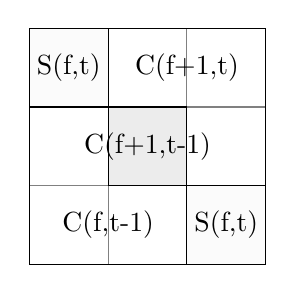
\begin{tikzpicture}
    \draw[step=1cm,color=gray] (0,0) grid (3,3);
    
    \draw[fill=gray!50, fill opacity=0.3] (1,1) -- (1,2) -- (2,2) -- (2,1) -- (1,1);
    \draw[fill=gray!10, fill opacity=0.3] (0,2) -- (0,3) -- (1,3) -- (1,2) -- (0,2);
    \draw[fill=gray!10, fill opacity=0.3] (2,0) -- (3,0) -- (3,1) -- (2,1) -- (2,0);
    
    
    \node[color=black] at (0.5,2.5) {S(f,t)};
    \node[color=black] at (2.5,0.5) {S(f,t)};
    \node at (1.5,1.5) {C(f+1,t-1)};
    
    
    
    \draw[color=black] (0,0) -- (0,2) -- (2,2) -- (2,0) -- (0,0);
    \draw[color=black] (3,3) -- (1,3) -- (1,1) -- (3,1) -- (3,3);
    
    \node[color=black] at (1,0.5) {C(f,t-1)};
    \node[color=black] at (2,2.5) {C(f+1,t)};
    
    \end{tikzpicture}
    \end{center}

\section{Computing Best Segmentation}\label{best_cost}

We obtain the cost of a full segmentation by summing the costs of its tracks. The goal is now to efficiently compute the segmentation of least cost.


A sequence $\t = (t_1, \ldots, t_{m+1})$ is called an $m/T$-segmentation if
\[
1 = t_1 < \ldots < t_m < t_{m+1} = T+1.
\]
$m$ is the number of tracks we are trying to find and is a parameter of the algorithm. We use the interpretation that track $i \in \{1, \ldots, m\}$ comprises times $\{t_i, \ldots, t_{i+1}-1\}$. Let $\segs^T_m$ be the set of all $m/T$-segmentations. Note that there is a very large number of possible segmentations 
\begin{multline*}
|\segs^T_m| ~=~ \binom{T-1}{m-1}
= \frac{(T-1)!}{(m-1)!(T-m)!} =\\
 \frac{(T-1)(T-2)\cdots(T-m+1)}{(m-1)!} \ge \left( \frac{T}{m}\right)^{m-1}.
\end{multline*} 
For large values of $T$, considering all possible segmentations using brute force is infeasible. For example, a two hour long show with $25$ tracks would have more than $\left( \frac{60^2 \times 2}{25}\right)^{24}  \approx 1.06 \times 10^{59}$ possible segmentations! 

We can reduce this number slightly by imposing upper and lower bounds on the song length.  Recall that $W$ is the upper bound (in seconds) of the song length, $w$ the lower bound (in seconds) and $m$ the number of tracks. With the track length restriction in place, the number of possible segmentations is still massive. A number now on the order of $10^{56}$ for a two hour show with $25$ tracks, $w=190$ and $W=60\times15$.



  Let $N(T,W,w,m)$ be the number of segmentations with time $T$ (in tiles),

We can write the recursive relation $$N(T,W,w,m) = \sum N(t_m-1,W,w,m-1)$$, where the sum is taken over $t_m$ such that 
\begin{align*}
t_m &\le T-w+1 & t_m &\ge T-W+1\\
t_m &\ge (m-1)w+1 & t_m &\le (m-1)W+1
\end{align*}

The first two inequalities mean that the length of the last track is within an acceptable boundary between $w$ and $W$. The last two inequalities mean that the lengths of the first $m-1$ tracks are within the same boundaries. 

We calculated the value of $N(7000, 60\times15, 190, 25)$ and got $5.20 \times 10^{56}$ which is still infeasible to compute with brute force.



Our solution to this problem is to find a dynamic programming recursion.

The loss of an $m/T$-segmentation $\t$ is 
\[
\loss(\t) 
~=~
\sum_{i=1}^m C(t_i, t_{i+1}-1)
\]
We want to compute
\[
\best^T_m ~=~ \min_{\t \in \segs^T_m} \loss(\t)
\]
To this end, we write the recurrence
\begin{equation*}
\best^t_1 ~=~ C(1, t) 
\end{equation*}
and for $i\ge2$
\begin{multline*}
\best^t_i ~=~
\min_{\t \in \segs^t_i} \loss(\t)
~=~ \min_{t_i} \min_{\t \in \segs^{t_i-1}_{i-1}} \loss(\t) + C(t_i, t)~=~  \\
\min_{t_i} C(t_i, t) + \min_{\t \in \segs^{t_i-1}_{i-1}} \loss(\t) 
~=~ \min_{t_i} C(t_i, t) + \best^{t_i-1}_{i-1}
\end{multline*}
%On page 7: t_i should range from t-W to t-w. It is about the position of the /last/ song.

In this formula $t_i$ ranges from $t-W$ to $t-w$. We have $T \times m$ values of $\best^T_m$ and calculating each takes at most $O(W)$ steps. The total time complexity is $O(TWm)$.

\begin{figure*}[t]
\centering
%\includegraphics[width=0.45\textwidth]{simmat_preds1.pdf}
%\hspace{1em}
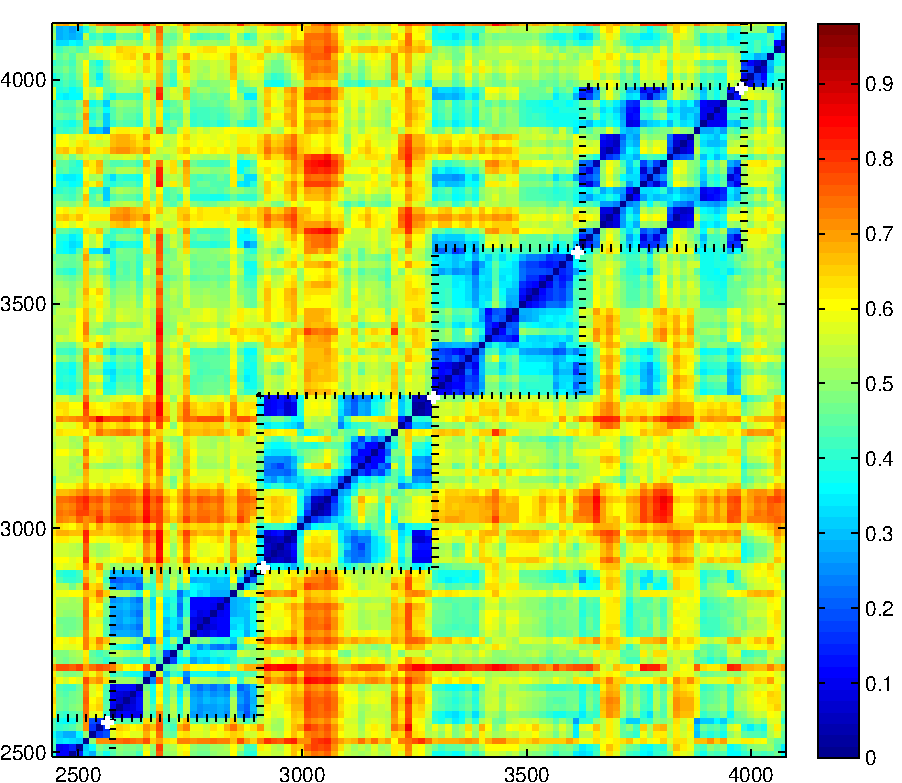
\includegraphics[width=\textwidth]{images/simmat_preds}

\caption{An illustration of what the dissimilarity matrix $S(i,j)$ looks like with the reconstructed indexes superimposed. White crosses indicate the human captured indices, and black dotted lines are the reconstructed indices. Note the error where one track has an end segment which is unlike the rest. }
\label{fig:predictions}
\end{figure*} 


 

\begin{table*}[f]
\centering
\caption {Main results. The accuracy rows show the mean of the absolute differences between the reconstructed tracks and the human indices (our test set). The thresholds indicate the percentage of reconstructed indices that fall within given time horizons centred around the actual indices. This is described in Section~\ref{eval_crit}.} \label{tab:mainresults} 
\vspace{1em}
{\setlength{\extrarowheight}{1.0pt}
\begin{tabular}{|l|l|l|l|l|l|}
\hline 
& \multicolumn{3}{c|}{\textbf{Dynamic By Show}}&  \multicolumn{2}{c|}{\textbf{Overall}}\\
\cline{2-6}
\multicolumn{1}{|>{\bf}l|}{}& {ASOT}& {TATW}& {MAGIC}& {Dynamic}& \multicolumn{1}{l|}{{Naive}}\\
 \hline 
\multicolumn{1}{|l|}{Number Shows}& 101& 89& 98& 288& \multicolumn{1}{l|}{288}\\
\hline 
\multicolumn{1}{|l|}{ 60 Seconds (\%) }& 92.3& 96.9& 97.9& 95.7& \multicolumn{1}{l|}{42.1}\\
\hline 
\multicolumn{1}{|l|}{ 30 Seconds (\%) }& 74.9& 90.4& 89.8& 85.1& \multicolumn{1}{l|}{22.0}\\
\hline 
\multicolumn{1}{|l|}{ 20 Seconds (\%) }& 63.7& 82.0& 74.4& 73.4& \multicolumn{1}{l|}{14.9}\\
\hline 
\multicolumn{1}{|l|}{ 10 Seconds (\%) }& 55.7& 70.9& 53.2& 59.9& \multicolumn{1}{l|}{7.6}\\
\hline 
\multicolumn{1}{|l|}{ 5 Seconds (\%) }& 43.9& 51.5& 32.9& 42.8& \multicolumn{1}{l|}{4.0}\\
\hline 
\multicolumn{1}{|l|}{ 3 Seconds (\%) }& 29.7& 35.3& 21.2& 28.7& \multicolumn{1}{l|}{2.6}\\
\hline 
\multicolumn{1}{|l|}{ 1 Second (\%) }& 11.6& 13.9& 8.3& 11.3& \multicolumn{1}{l|}{0.9}\\
\hline 
\multicolumn{1}{|l|}{Accuracy (Seconds)}& 49.4& 40.1& 26.5& 38.6& \multicolumn{1}{l|}{112.2}\\
\hline 
\end{tabular}}

\end{table*}

\begin{table}
\centering
\caption {Results for the pruned set of shows (that do not contain tracks smaller than $180$ seconds). The percentage figure given on the number of shows indicates how many were discarded from the prune. Performance on TATW and Magic Island are robustly improved. Magic Island achieved the improvement with a comparatively small prune of 7.4\%.} \label{tab:prunedresults} 
\vspace{1em}
{\setlength{\extrarowheight}{1.0pt}
\begin{tabular}{|l|l|l|l|l|l|}
\hline 
& \multicolumn{3}{c|}{\textbf{Dynamic By Show}}&  \multicolumn{2}{c|}{\textbf{Overall}}\\
\cline{2-6}
\multicolumn{1}{|>{\bf}l|}{}& {ASOT}& {TATW}& {MAGIC}& {Dynamic}& \multicolumn{1}{l|}{{Naive}}\\
\hline 
\multicolumn{1}{|l|}{Number Shows}& 64 (42.3\%) & 61 (38.4\%) & 100 (7.4\%) & 225& \multicolumn{1}{l|}{288}\\
\hline 
\multicolumn{1}{|l|}{ 60 Seconds (\%) }& 93.4& 98.2& 98.9& 96.8& \multicolumn{1}{l|}{42.1}\\
\hline 
\multicolumn{1}{|l|}{ 30 Seconds (\%) }& 75.7& 92.3& 90.8& 86.2& \multicolumn{1}{l|}{22.0}\\
\hline 
\multicolumn{1}{|l|}{ 20 Seconds (\%) }& 63.5& 84.0& 74.9& 74.1& \multicolumn{1}{l|}{14.9}\\
\hline 
\multicolumn{1}{|l|}{ 10 Seconds (\%) }& 56.3& 72.8& 53.2& 60.8& \multicolumn{1}{l|}{7.6}\\
\hline 
\multicolumn{1}{|l|}{ 5 Seconds (\%) }& 44.0& 52.8& 32.6& 43.2& \multicolumn{1}{l|}{4.0}\\
\hline 
\multicolumn{1}{|l|}{ 3 Seconds (\%) }& 30.0& 36.5& 20.9& 29.1& \multicolumn{1}{l|}{2.6}\\
\hline 
\multicolumn{1}{|l|}{ 1 Second (\%) }& 12.1& 15.2& 8.6& 12.0& \multicolumn{1}{l|}{0.9}\\
\hline 
\multicolumn{1}{|l|}{Accuracy (Seconds)}& 32.3& 14.9& 13.3& 20.2& \multicolumn{1}{l|}{112.2}\\
 \hline 
\end{tabular}}

\end{table}

\section{Improved Cost Function Ideas}\label{sec:improved-cost-function-ideas}

See Figure~\ref{fig:costfailing} for an illustration of where the previous cost function would run into problems. When you have a track structure \{A,B,A\}, the previous cost function result would depend on the similarity of A and B. The track in the diagram is an extreme example of when A and B are completely different. This should not in principle reduce the likelihood of placing a track.

So what is an improved cost function? Here are some ideas to motivate further work.

1. We are interested in similarity more than than dissimilarity. 
 
2. We are also interested in the self-similarity distance, a highly self-similar region far away is a strong signal, even if entirely disconnected i.e. no interim regions of the same type.

3. We want to reward contiguity. The longer the better and the further into the future, the better, perhaps with some limit. A Gaussian could be fit to describe the optimum time horizon of self-similarity. 

4. Some kind of time derivative, looking for a straight edge in the similarity matrix. High deltas should be rewarded. 

5. Perhaps it would be possible to transform the information in $S$ for a corresponding $C(t,f)$ out of the time domain before evaluation to remove the $\{ABA\}$ dependency. 







\section{Posterior Marginal of Song Boundary}
Fix a learning rate $\eta$, and fix $T$ and $M$. Let
\[
P(j,s) ~=~ 
\frac{\displaystyle
\sum_{\t \in \segs^T_m : t_j = s} e^{- \eta \loss(\t)}
}{\displaystyle
\sum_{\t \in \segs^T_m} e^{- \eta \loss(\t)}
}
\]
That is, $P(j,s)$ is the ``posterior probability'' that song $j$ starts at time $s$.

To compute $P(j,s)$, we need an extended notion of segmentation. We call $\t$ a $m/F: T$ segmentation if
\[
F = t_1 < \ldots < t_m < t_{m+1} = T+1.
\]
Let $\segs^{F : T}_m$ be the set of all $m/F-T$-segmentations. 
%
We have
\[
\sum_{\t \in \segs^T_m : t_j = s} e^{- \eta \loss(\t)}
~=~
\sum_{\t \in \segs^{s-1}_{j-1}, \t' \in \segs^{s : T}_{m-j+1}} e^{- \eta (\loss(\t) +\loss(\t'))}
~=~
\left(\sum_{\t \in \segs^{s-1}_{j-1}} e^{- \eta \loss(\t)}\right)
\left(\sum_{\t \in \segs^{s : T}_{m-j+1}} e^{- \eta \loss(\t)}\right)
\]
%
which upon abbreviating
\begin{align*}
\head^t_m & ~=~ \sum_{\t \in \segs^{t}_{m}} e^{- \eta \loss(\t)} &
\tail^f_m & ~=~ \sum_{\t \in \segs^{f : T}_m} e^{- \eta \loss(\t)}
\end{align*}
means that we can write
\[
P(j,s) ~=~ \frac{\head^{s-1}_{j-1} \cdot \tail^{s}_{m-j+1}}{\head^T_m}
.
\]
So it suffices to compute $\head^{t}_{m}$ and $\tail^{t}_{m}$ for all relevant $t$ and $m$. We use
\begin{align*}
\head^t_1 &~=~ e^{-\eta C(1,t)} &
\tail^f_1 &~=~ e^{- \eta C(f, T-f+1)}
\intertext{and for $m\ge2$}
\head^t_m 
&~=~ 
\sum_{t_m} \sum_{\t \in \segs^{t_m-1}_{m-1}} e^{- \eta (\loss(\t) + C(t_m, t-t_m+1))} 
&
\tail^f_m 
&~=~ 
\sum_{t_2} \sum_{\t \in \segs^{t_2 : T}_{m-1}} e^{- \eta (C(f, t_2-f) + \loss(\t))}
\\
&~=~ 
\sum_{t_m} e^{-\eta C(t_m, t-t_m+1)} \sum_{\t \in \segs^{t_m-1}_{m-1}} e^{- \eta \loss(\t)}
&
&~=~
\sum_{t_2} e^{- \eta C(f, t_2-f)} \sum_{\t \in \segs^{t_2 : T}_{m-1}} e^{- \eta \loss(\t)}
\\
&~=~ 
\sum_{t_m} e^{-\eta C(t_m, t-t_m+1)} \head^{t_m-1}_{m-1}
&
&~=~
\sum_{t_2} e^{- \eta C(f, t_2-f)} \tail^{t_2}_{m-1}
\end{align*}



\section{Posterior Marginal of Song Position}
Fix a learning rate $\eta$, and fix $T$ and $M$. Let
\[
P(j,s,f) ~=~ 
\frac{\displaystyle
\sum_{\t \in \segs^T_m : t_j = s \land t_{j+1}-1 = f} e^{- \eta \loss(\t)}
}{\displaystyle
\sum_{\t \in \segs^T_m} e^{- \eta \loss(\t)}
}
\]
That is, $P(j,s,f)$ is the ``posterior probability'' that song $j$ starts at time $s$ and finishes at time $f$.
%
In the same vein as the last section, we now get
\[
P(j,s,f) ~=~ \frac{\head^{s-1}_{j-1} \cdot e^{-\eta C(s, f-s+1)} \cdot \tail^{f+1}_{m-j}}{\head^T_m}.
\]


\section{Summary}\label{conclusions}

We believe our algorithm would be useful for segmenting DJ-mixed audio streams in batch mode. Our overall average is encouraging, taking into account the difficulty of the task at hand. The dissimilarity matrix we use is based solely on instrument features. The most pervasive elements in EDM are the percussion (the beats). We believe on balance that ignoring the percussive information was advantageous, because DJs use percussion primarily to blur boundaries between tracks.  We tried to capture percussive based features and found that the transitions between tracks and indeed groups of tracks appeared as stronger self-similar regions in $S$ than the actual tracks. We captured the percussive features by taking the cross correlation of the samples in the time domain, and using the same convolution filter. See Figure~\ref{fig:xcorr} for an illustration of why percussion features were not as good as instrumental features for this domain.

%maybe update this now
We would like to improve our cost function with one that has some domain knowledge, perhaps using a machine learning algorithm. Currently our cost function has a weakness that the relative similarity of regions within a song matters slightly, it should be independent. Let us consider the song structure \{A,B,A\}. The problem is that our cost (summing/normalizing the $S$ square) would somewhat take into consideration the similarity of A and B. Anyone interested in optimizing the algorithm for a one specific radio show could consider modifying the cost function to introduce a parameter $\alpha \in [0,1]$ for fine tuned control over the normalization bias placed on the length of songs; $C(f,t) ~=~ \frac{ \sum_{i=f}^{t} \sum_{j=f}^{t} S(i,j) }{ (t-f+1)^\alpha }$. 

 We would also like to implement some of the methods in the literature (which were mostly designed for scene analysis) to see if we outperform them. It would be tricky to get an exact comparison because we could not find a unsupervised deterministic algorithm which finds a fixed number of strictly contiguous clusters. We could however adapt existing algorithms to get a like for like comparison. We would like to evaluate the performance of J Theiler's contiguous K-means algorithm in particular \cite{theiler1997contiguity} and also similar algorithms. We have the property of being deterministic but probabilistic methods should be explored. Theiler's algorithm would require some modification to work in this scenario because we require strictly contiguous clusters, not just a contiguity bias. 







\bibliographystyle{ieeetr}
\bibliography{bib/references,bib/refs}

\end{document}
